%!TEX root = ../Thesis.tex
\section{Skip-gram}

The skip-gram mtodel doesn't need to be trained as there exists a pre trained version at \url{https://code.google.com/p/word2vec/}. This pre trained version has a latent size of 300 dimensions. The weights are trained using the Google News dataset, which is about 100 billion words and unfortunately not publicly available.

The document vectors are then constructed by taking the average sum over all the word vectors. Using the full text of each article is unlikely to provide any good results, as there would be a lot of irrelevant words which would create a lot of noise. 

Instead just the title of the article is used and as an experiment the title and the lead is also considered.

\paragraph{Document vectors} Using principal component analysis the vector representations of all the documents can be visualized in both cases.
\begin{figure}[H]
	\centering
	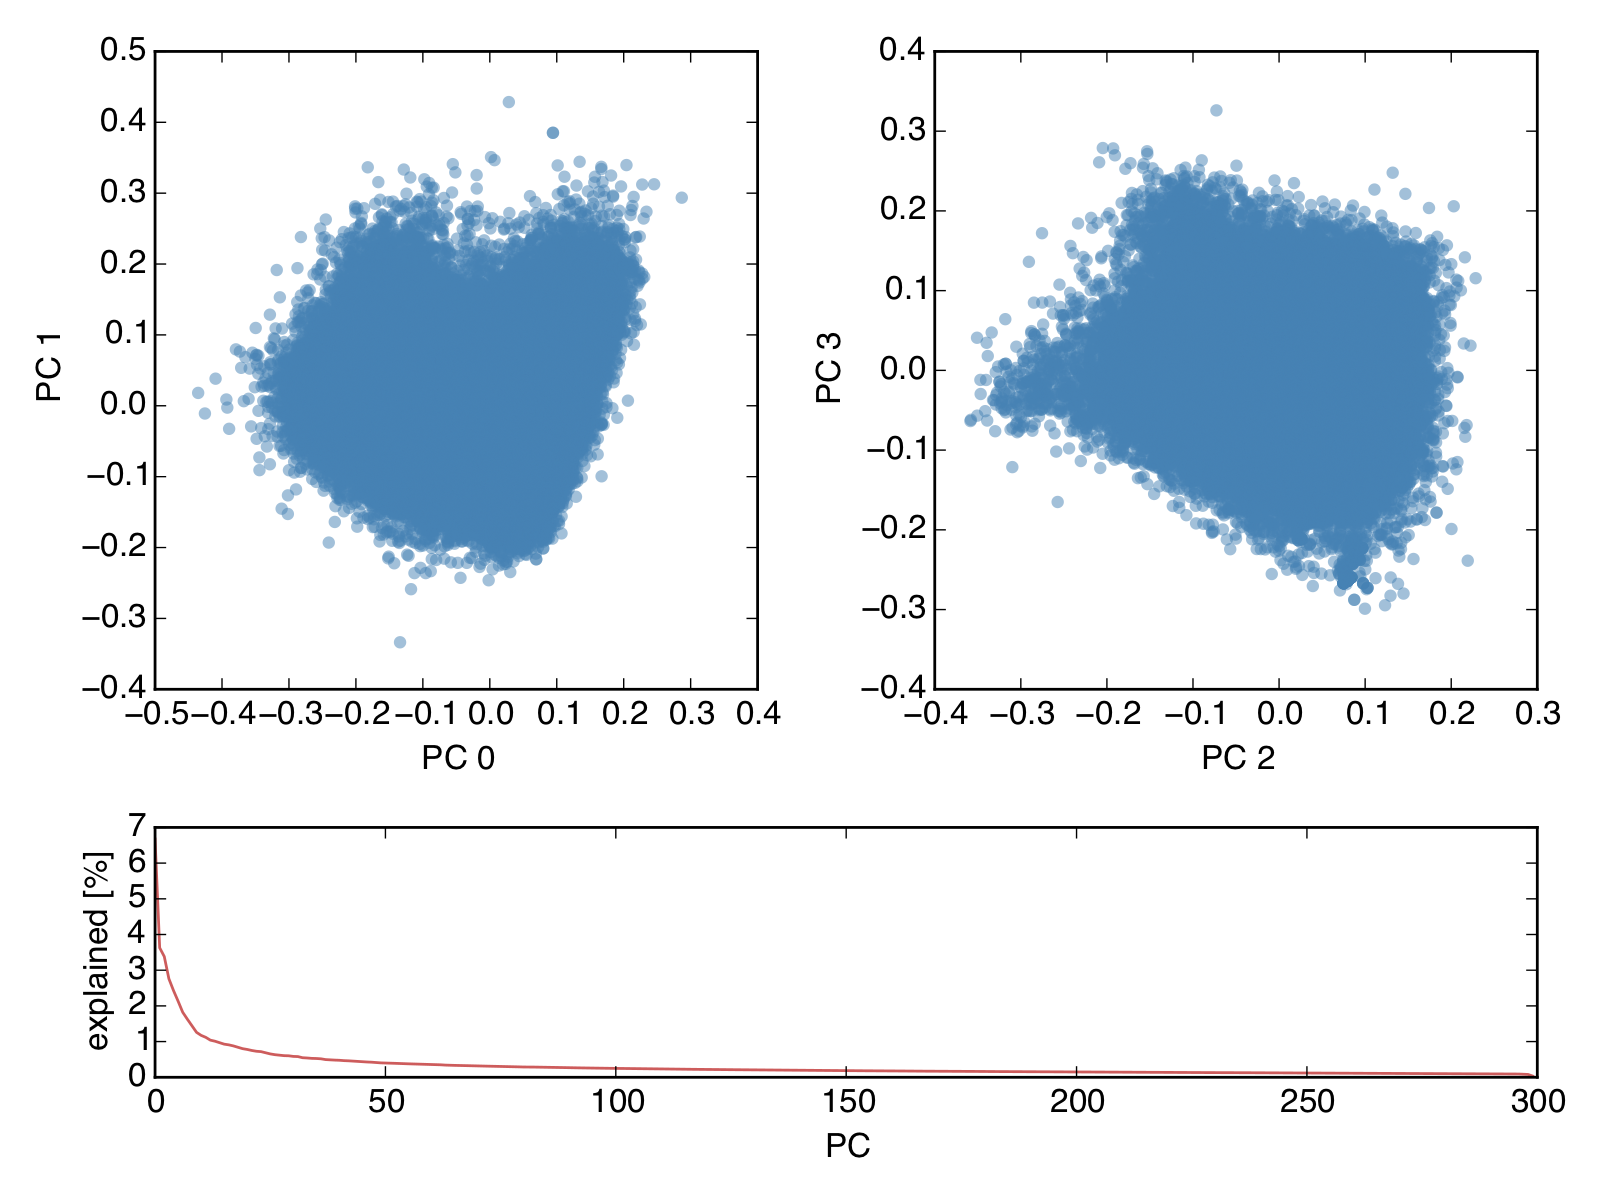
\includegraphics[width=0.9\textwidth]{results/word2vec-title-pca}
	\caption{Document vectors calculated from just the title. Explained variance on the first 4 principal components is 16.4\%.}
\end{figure}

\begin{figure}[H]
	\centering
	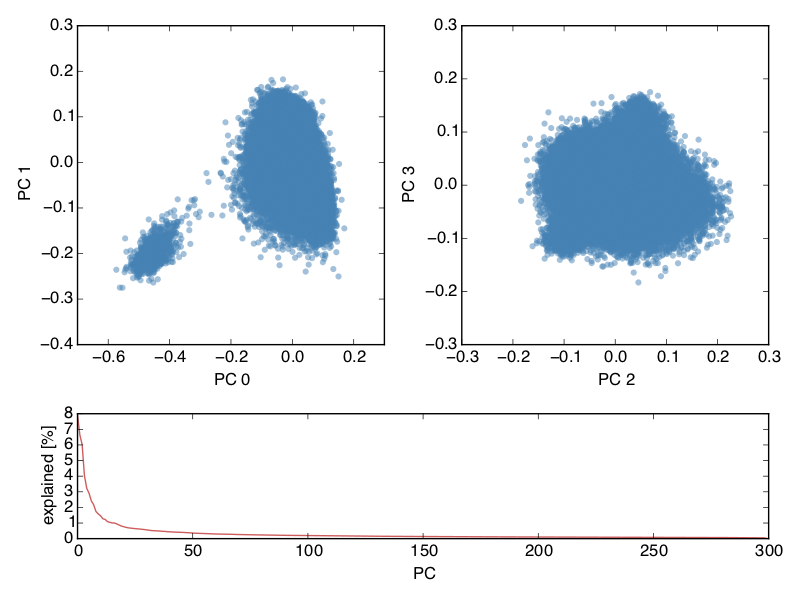
\includegraphics[width=0.9\textwidth]{results/word2vec-both-pca}
	\caption{Document vectors calculated from both title and lead. Explained variance on the first 4 principal components is 24.6\%.}
\end{figure}

Without any labeling of the documents the scatter plots are not very informative. The explained variance score is not very high compared to what one usually observes on raw data. This indicated the skip-gram model is somewhat effective in generating descriptive document vectors there aren't too correlated.

An interesting result is that the first principal component seams to contain two big clusters of documents. However by inspecting some of the nodes there do not appear to be any reason for this separation.

\paragraph{Distance histogram} Since a distance measure will be used to perform the clustering, it makes sense to inspect the histogram of the distance measures. Note that only distances between nodes there are connected by the chronological connectivity matrix have been calculated.

The density estimation required for showing the histogram, also serves the purpose of providing the basis for calculating a somewhat consistent threshold across the different experiments. The threshold $t$ is chosen a the $0.1 \%$ percentile, that is $P(distance < t) = 0.001$. This percentile was chosen qualitatively by running a few experiments, but it turns out it doesn't matter much, as the threshold is not the bottleneck of the performance.

\begin{figure}[H]
        \centering
        \begin{subfigure}[b]{0.49\textwidth}
                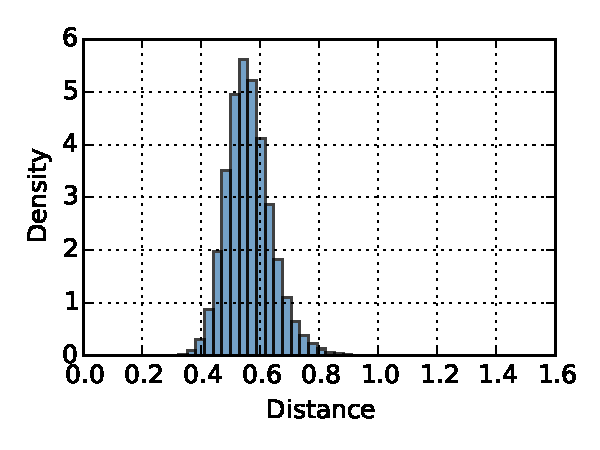
\includegraphics[width=\textwidth]{results/word2vec-title-l2-histogram}
                \caption{Euclidean distance ($t \approx 0.35$)}
        \end{subfigure}
        \begin{subfigure}[b]{0.49\textwidth}
                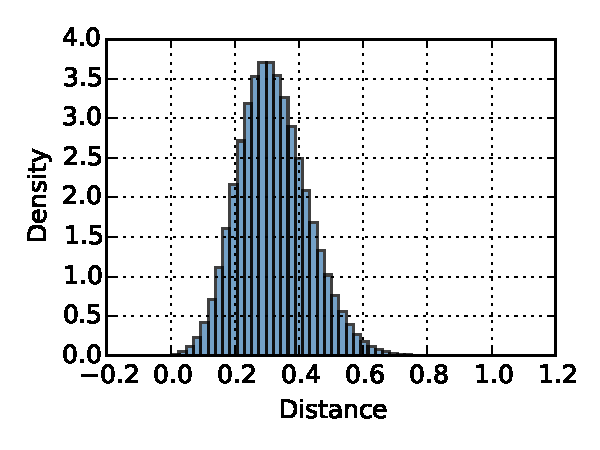
\includegraphics[width=\textwidth]{results/word2vec-title-cos-histogram}
                \caption{Cosine similarity ($t \approx 0.14$)}
        \end{subfigure}
        \caption{Histograms of the distance values using just the title for generating document vectors.}
\end{figure}
\begin{figure}[H]
        \centering
        \begin{subfigure}[b]{0.49\textwidth}
                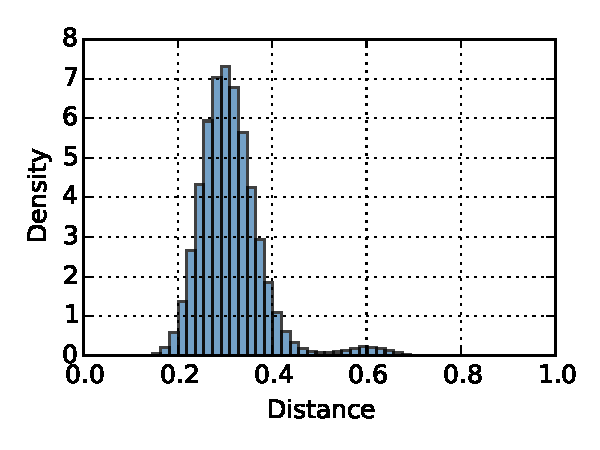
\includegraphics[width=\textwidth]{results/word2vec-both-l2-histogram}
                \caption{Euclidean distance ($t \approx 0.14$)}
        \end{subfigure}
        \begin{subfigure}[b]{0.49\textwidth}
                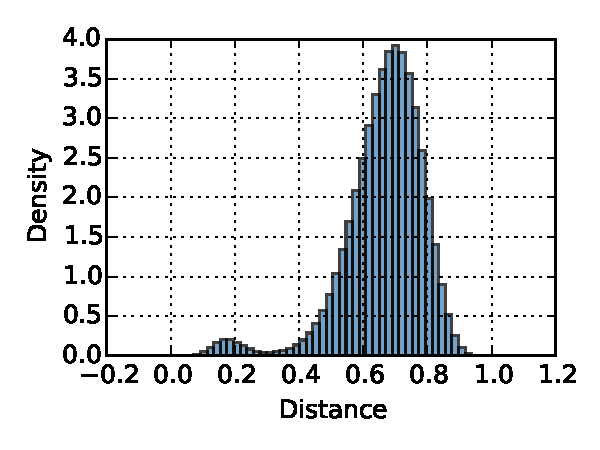
\includegraphics[width=\textwidth]{results/word2vec-both-cos-histogram}
                \caption{Cosine similarity ($t \approx 0.092$)}
        \end{subfigure}
        \caption{Histograms of the distance values using both title and lead for generating document vectors.}
\end{figure}

The histograms shows the distances are approximately normally distributed. This is not very surprising as the both the euclidean distance and cosine similarly involves a large sum and thus have relations to the central limit theorem.

\paragraph{Inspecting clusters}  None of the 4 variations gives particularly good results. They all cluster the documents such that there is a ridiculously huge amount of unique articles. This alone could indicate the threshold is too small. However simultaneously they all have cluster really big clusters, with up to $31478$ documents in one case. Because there exists clusters that either way to big or way to small, the threshold is not the problem. It is the skip-gram model or perhaps the clustering method there causes the bad results.

\begin{table}[H]
\centering
\begin{tabular}{r|l l l l l l }
size & 1 & 2 & 81 & 318 & 715 & 17023 \\ \hline
amount & 81857 & 3 & 1 & 1 & 1 & 1
\end{tabular}
\caption{Example of the cluster size distribution. In this case both article title and article lead was used for generating document vectors and cosine similarity was used for clustering. Note that using euclidean distance yields way more reasonably sized clusters.}
\end{table}

It should be noted that some clusters do provide good results:

\begin{table}[H]
\centering
\begin{tabular}{r|p{10cm}}
id & title \\ \hline
 25167 & Teenage stowaway survives five-hour flight hiding in wheel of plane \\
 25354 & Survival of teenage stowaway on five-hour flight to Hawaii is medical 'miracle', say experts \\
 25140 & Teenager stowaway 'survives five-hour flight in wheel of plane' \\
 26276 & How teenage boy stowed away on plane wheel well \\
 25567 & Teenage stowaway survives five-hour flight in jet's wheel
\end{tabular}
\caption{A cluster containing articles about the same story. Produced using euclidean distance on document vectors produced from both title and lead.}
\end{table}
 
Similar results can be found when just looking at the title and using euclidean distance for clustering. However using cosine similarity did not yield any meaningful results, independent of whether or not the article lead was included. This is wired as the skip-gram papers \cite{word2vec-comparing, word2vec-details} uses the cosine similarity for finding similar words. It could be because cosine similarity is usually used in a context where the length of the vector isn't important. But in this case having a big length could indicate how extreme the article is in its language, which could be created to the story. 
